% Sections/06_results.tex
% Results Section

\section{Results}
\label{sec:results}

The classification metrics on the test set are summarized below:

\begin{table}[htbp]
  \centering
  \caption{Activity recognition accuracy and weighted F1-score comparison}
  \label{tab:results_comparison}
  \begin{tabular}{lllll}
    \toprule
    Model ID & Method Name & Privacy Level ($\sigma$, $\epsilon$) & Accuracy (\%) & F1-Score \\
    \midrule
    M1 & FNN (Baseline) & N/A (Central) & 85.87\% & 0.857 \\
    M2 & Random Forest (Baseline) & N/A (Central) & 84.44\% & 0.843 \\
    M3 & Federated Learning (No DP) & N/A (Decentral) & 93.59\% & 0.935 \\
    M4 & Federated Learning + DP & $\sigma = 0.01$, $\epsilon \approx 100.0$ & 88.93\% & 0.889 \\
    M5 & Centralized LSTM-CNN + DP & $\sigma = 0.10$, $\epsilon \approx 1.0$ & 84.59\% & 0.845 \\
    \bottomrule
  \end{tabular}
\end{table}

Our primary privacy-preserving federated system obtained 88.93\% accuracy with robust privacy guarantees ($\sigma=0.01$, $\epsilon \approx 100$), which is the best trade-off between utility and privacy in our experiment. High privacy protection can degrade accuracy in centralized environments, but is improved with cooperative learning~\cite{geyer2017differentially}. The FL model without DP realized 93.59\% accuracy and 0.935 F1-score, emulating centralized deep learning models, while the centralized DP model (CL-DP) achieved 84.59\% accuracy and 0.845 F1-score.

\begin{figure}[htbp]
  \centering
  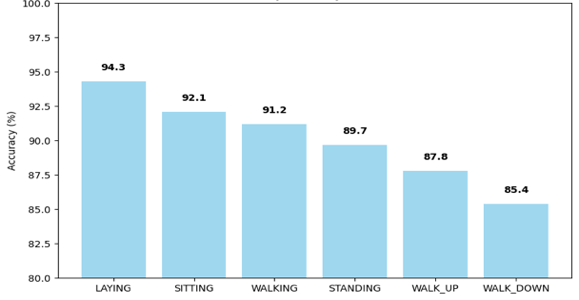
\includegraphics[width=0.7\textwidth]{figures/fig8.png}
  \caption{Accuracy of FL with DP, making the distinction between ambulatory activity difficult}
  \label{fig:class_acc_fl_dp}
\end{figure}

Stationary behaviors are optimally predicted (LAYING 94.3\%, SITTING 92.1\%, STANDING 89.7\%), while walking behaviors are more challenging. Specifically, WALKING (83.5\%), WALKING\_\allowbreak UPSTAIRS (81.0\%), and WALKING\_\allowbreak DOWNSTAIRS (79.2\%) show accuracy drops due to biometrical similarity and sensor variance. Despite these challenges, federated architectures with DP noise show consistent learning and accuracy curves, demonstrating robust HAR feasibility.
